%----------------------------------------------------------------------------------------
%	PACKAGES AND OTHER DOCUMENT CONFIGURATIONS
%----------------------------------------------------------------------------------------

\documentclass[a0,portrait]{a0poster}

\usepackage{multicol} % This is so we can have multiple columns of text side-by-side
\columnsep=100pt % This is the amount of white space between the columns in the poster
\columnseprule=3pt % This is the thickness of the black line between the columns in the poster

\usepackage[svgnames]{xcolor} % Specify colors by their 'svgnames', for a full list of all colors available see here: http://www.latextemplates.com/svgnames-colors

\usepackage{times} % Use the times font
%\usepackage{palatino} % Uncomment to use the Palatino font

\usepackage{graphicx} % Required for including images
\graphicspath{{figures/}} % Location of the graphics files
\usepackage{booktabs} % Top and bottom rules for table
\usepackage[font=small,labelfont=bf]{caption} % Required for specifying captions to tables and figures
\usepackage{amsfonts, amsmath, amsthm, amssymb} % For math fonts, symbols and environments
\usepackage{wrapfig} % Allows wrapping text around tables and figures

\usepackage{mathpartir}
\usepackage{xspace}
\usepackage{stmaryrd}
\usepackage{listings}
\usepackage{newtxmath}

%% Tikz Needed packages
\usepackage{pgfplots}
\pgfplotsset{width=7cm,compat=1.8}
\usepackage{pgfplotstable}
\renewcommand*{\familydefault}{\sfdefault}

\newcommand{\lang}{\textsc{Effy}\xspace}
\newcommand{\eff}{\textsc{Eff}\xspace}
\newcommand{\ocaml}{\textsc{OCaml}\xspace}

% Meta-syntax
\newcommand{\bnfis}{\mathrel{\;{:}{:}\!=}\;}
\newcommand{\bnfor}{\mathrel{\;|\;}}
\newcommand{\defeq}{\mathrel{\;\stackrel{\text{def}}{=}\;}}
\newcommand{\set}[1]{\{ #1 \}}

% General syntactic constructs
\newcommand{\kord}[1]{\mathtt{#1}}
\newcommand{\kop}[1]{\;\mathtt{#1}\;}
\newcommand{\kpre}[1]{\mathtt{#1}\;}
\newcommand{\kpost}[1]{\;\mathtt{#1}}

% Types
\newcommand{\type}[1]{\mathtt{#1}}
\newcommand{\boolty}{\type{bool}}
\newcommand{\intty}{\type{int}}
\newcommand{\hto}{\Rightarrow}
\renewcommand{\C}{\underline{C}}
\newcommand{\D}{\underline{D}}
\newcommand{\dirt}{\Delta}
\newcommand{\sig}{\Sigma}

% Expressions and computations
\newcommand{\funtyped}[2]{\kpre{fun} #1 \T #2 \mapsto}

\newcommand{\call}[3]{{{#1}\,{#2}\,{#3}}}
\newcommand{\case}{\mathop{\text{\texttt{|}}}}
\newcommand{\cont}[2]{(#1.\,#2)}
\newcommand{\const}{\kord{k}}
\newcommand{\fls}{\kord{false}}
\newcommand{\fun}[1]{\kpre{fun} #1 \mapsto}
\newcommand{\handler}[1]{\{ #1 \}}
\newcommand{\conditional}[3]{\kpre{if} #1 \kop{then} #2 \kop{else} #3}
\newcommand{\letin}[1]{\kpre{let} #1 \kop{in}}
\newcommand{\doin}[1]{\kpre{do} #1 \kop{ ; }}
\newcommand{\letrecin}[1]{\kpre{let} \kpre{rec} #1 \kop{in}}
\newcommand{\op}{\kord{Op}}
\newcommand{\ops}{\mathcal{O}}
\newcommand{\ocs}{\mathit{ocs}}
\newcommand{\ocsnil}{\kord{nil}}
\newcommand{\tru}{\kord{true}}
\newcommand{\ret}{\kpre{return}}
\newcommand{\withhandle}[2]{\kpre{handle} #2 \kop{with} #1}
\newcommand{\pure}[1]{\kord{pure } #1  }
\newcommand{\longcases}{\call{\op_1}{y}{k} \mapsto c_{\op_1}, \ldots, \call{\op_n}{x}{k} \mapsto c_{\op_n}}
\newcommand{\shortcases}{[\call{\op}{y}{k} \mapsto c_\op]_{\op \in \ops}}
\newcommand{\longhand}[1][\ret x \mapsto c_r]{\handler{#1, \longcases}}
\newcommand{\shorthand}[1][\ret x \mapsto c_r]{\handler{#1, \shortcases}}

% Type-checking
\newcommand{\row}{\mathrel{;} R}
\newcommand{\ctx}{\Gamma}
\newcommand{\ent}{\vdash}
\newcommand{\T}{\mathrel{:}}
\newcommand{\E}{\mathrel{!}}
\newcommand{\covers}{\mathrel{/}}
\renewcommand{\le}{\leqslant}

% Operational semantics
\newcommand{\eval}{\Downarrow}
\newcommand{\hs}{\mathcal{H}}
\newcommand{\nil}{\emptyset}
\newcommand{\cons}{\mathbin{::}}
\newcommand{\hseval}[1][\hs]{\Downarrow_{#1}}
\newcommand{\getval}[1]{{#1}_{\kord{val}}}
\newcommand{\getop}[1]{{#1}_{\kord{op}}}


\begin{document}

%----------------------------------------------------------------------------------------
%	POSTER HEADER 
%----------------------------------------------------------------------------------------

\begin{minipage}[b]{0.70\linewidth}
\veryHuge \color{NavyBlue} \textbf{Towards a core language with row-based effects for optimised compilation} \color{Black}\\ % Title
%\Huge\textit{An Exploration of Complexity}\\[2cm] % Subtitle
\huge \textbf{Axel Faes - Advised by: Tom Schrijvers}\\[0.5cm] % Author(s)
\huge KULeuven - Computer Science\\[0.4cm] % University/organization
%\Large \texttt{john@LaTeXTemplates.com} --- 1 (000) 111 1111\\
\end{minipage}
%
\begin{minipage}[b]{0.30\linewidth}

\includegraphics[width=20cm]{logo.png}\\
\end{minipage}

\vspace{1cm} % A bit of extra whitespace between the header and poster content

%----------------------------------------------------------------------------------------

\begin{multicols}{2} % This is how many columns your poster will be broken into, a portrait poster is generally split into 2 columns

%----------------------------------------------------------------------------------------
%	ABSTRACT
%----------------------------------------------------------------------------------------

\color{Navy} % Navy color for the abstract

\begin{abstract}
Algebraic effects and handlers are a very active area of research. An important aspect is the development of an optimising compiler. \eff is an ML-style language with support for effects and forms the testbed for the optimising compiler. However, \eff does not offer explicit typing, which makes it easy for type checking bugs to be introduced during the construction of optimised compilation. This work presents a new core language with row-based effects. The core language is explicitly typed in order to reduce bugs in the optimised compilation.
\end{abstract}

%----------------------------------------------------------------------------------------
%	INTRODUCTION
%----------------------------------------------------------------------------------------

\color{SaddleBrown} % SaddleBrown color for the introduction

\section*{Introduction}
Algebraic effect handling is a very active area of research. Implementations of algebraic effect handlers are becoming available. Because of this, improving performance is becoming the focus of research. A lot of research focusses on speeding up the runtime performance. However, a runtime penalty still occurs. This happens since handlers or continuations need to be repeatedly copied on the heap. Due to this, we are looking towards type-directed optimised compilation of algebraic effect handlers. We want to remove the handlers such that no copying is required and thus no runtime penalty occurs. \\
\\
In our ongoing research towards type-directed optimised compilation, term rewrite rules and purity aware compilation optimise away most handlers. Term rewrite rules use information of the type-\&-effect system. Term rewrite rules perform two types of actions. They remove handlers and apply effects such that eventually the program does not contain any more handlers. Term rewrite rules can also change the syntactic structure in order to expose more possibilities for optimisations. Purity aware compilation identifies computations that are effectively pure and purifies them.  \\
\\
\eff, an ML-style language, is being used to develop an optimised compiler for algebraic effect handlers. \eff uses a type system based on subtyping \cite{effectsystem}. As explained by Bauer and Pretnar in \cite{programming}, terms in \eff do not contain any information about computational effects. This information has to be inferred using type inference algorithms. The lack of explicit type information makes source-to-source transformations much more error-prone. Additionally, ensuring that a transformation does not break typeability becomes a time-consuming task, since we need to reconstruct types after each optimisation pass. \\
\\
The current type system with subtyping becomes impractical since the typing information is not explicitly contained in each term. There are several solutions to make the type system more practical. It is possible to keep subtyping, but use a unification based algorithm \cite{mlsub}. Implicit effect polymorphism can also be used \cite{impliciteff}. The option that is explored in this work, is to use a simple type-\&-effect system based on row-polymorphism \cite{type-directed, leijen2014koka, row}. \\
\\
In this work, we present a simple explicitly-typed language that can serve as an intermediate language during compilation of \eff, and allows for the development of type-preserving core-to-core transformations. Optimisation and term rewriting is done using this core language. This approach will ease the development of an optimised compiler since typechecking becomes linear due to the explicit typing.

%----------------------------------------------------------------------------------------
%	OBJECTIVES
%----------------------------------------------------------------------------------------

\color{DarkSlateGray} % DarkSlateGray color for the rest of the content

\section*{Main Objectives}

%\begin{enumerate}
%\item Lorem ipsum dolor sit amet, consectetur.
%\item Nullam at mi nisl. Vestibulum est purus, ultricies cursus volutpat sit amet, vestibulum eu.
%\item Praesent tortor libero, vulputate quis elementum a, iaculis.
%\item Phasellus a quam mauris, non varius mauris. Fusce tristique, enim tempor varius porta, elit purus commodo velit, pretium mattis ligula nisl nec ante.
%\item Ut adipiscing accumsan sapien, sit amet pretium.
%\item Estibulum est purus, ultricies cursus volutpat
%\item Nullam at mi nisl. Vestibulum est purus, ultricies cursus volutpat sit amet, vestibulum eu.
%\item Praesent tortor libero, vulputate quis elementum a, iaculis.
%\end{enumerate}

%----------------------------------------------------------------------------------------
%	MATERIALS AND METHODS
%----------------------------------------------------------------------------------------

\section*{Background}


%\begin{figure}[h]
\begin{center}
\framebox{
\begin{minipage}{0.98\columnwidth}
\[\begin{array}{r@{~}c@{~}l@{\quad}l}
  \text{value}~v & \bnfis {} & x & \text{variable} \\
    & \bnfor & \const & \text{constant} \\
    & \bnfor & \fun{x} c & \text{function} \\
    & \bnfor & \{ & \text{handler} \\
    & & \quad \ret x \mapsto c_r, & \quad\text{return case} \\
    & & \quad \shortcases & \quad\text{operation cases} \\
    & & \} & \\
  \text{comp}~c & \bnfis & v_1 \, v_2 & \text{application} \\
    & \bnfor & \letrecin{f \, x = c_1} c_2 & \text{rec definition} \\
    & \bnfor & \ret v  & \text{returned val} \\
    & \bnfor & \op \, v & \text{operation call} \\
    & \bnfor & \doin{x \leftarrow c_1} c_2 & \text{sequencing} \\
    & \bnfor & \withhandle{v}{c} & \text{handling}
\end{array}\]
\end{minipage}
}
\end{center}
%\caption{Terms of \eff as described in previous work}\label{fig:terms:eff}
%\end{figure}

%\begin{figure}
\begin{center}
\framebox{
\begin{minipage}{0.98\columnwidth}
\[\begin{array}{r@{~}c@{~}l@{\quad}l}
  \text{(pure) type}~A, B & \bnfis {}
    & \boolty \bnfor \intty & \text{basic types} \\
    & \bnfor & A \to \C & \text{function type} \\
    & \bnfor & \C \hto \D & \text{handler type} \\
  \text{dirty type}~\C, \D & \bnfis {} & A \E \dirt \\
  \text{dirt}~\dirt & \bnfis {} &\set{\op_1, \dots, \op_n}
\end{array}\]
\end{minipage}
}
\end{center}
%\caption{Types of \eff as described in previous work}\label{fig:types:eff}
%\end{figure}

%\begin{figure}[h]
\begin{center}
\framebox{
\begin{minipage}{0.98\columnwidth}
\[\begin{array}{r@{~}c@{~}l@{\quad}l}
  \text{value}~v & \bnfis {} & x & \text{variable} \\
    & \bnfor & \const & \text{constant} \\
    & \bnfor & \lambda (x : A). c & \text{\textbf{function}} \\
    & \bnfor & \Lambda \alpha . c & \text{\textbf{type abstraction}} \\
    & \bnfor & \{ & \text{handler} \\
    & & \quad \ret x \mapsto c_r, & \quad\text{return case} \\
    & & \quad \shortcases & \quad\text{operation cases} \\
    & & \} & \\
  \text{comp}~c & \bnfis & v_1 \, v_2 & \text{application} \\
    & \bnfor & v \, A & \text{\textbf{type application}} \\
    & \bnfor & \letrecin{f \, x = c_1} c_2 & \text{rec definition} \\
    & \bnfor & \ret v  & \text{returned val} \\
    & \bnfor & \op \, v & \text{operation call} \\
    & \bnfor & \doin{x \leftarrow c_1} c_2 & \text{sequencing} \\
    & \bnfor & \withhandle{v}{c} & \text{handling}
\end{array}\]
\end{minipage}
}
\end{center}
%\caption{Terms of the explicitly typed core language}\label{fig:terms:explicit}
%\end{figure}

%\begin{figure}
\begin{center}
\framebox{
\begin{minipage}{0.98\columnwidth}
\[\begin{array}{r@{~}c@{~}l@{\quad}l}
  \text{(pure) type}~A, B & \bnfis {}
    & A \to \C & \text{function type} \\
    & \bnfor & \C \hto \D & \text{handler type} \\
    & \bnfor & \alpha & \text{\textbf{type variable}} \\
    & \bnfor & \forall \alpha . \C & \text{\textbf{polytype}} \\
  \text{dirty type}~\C, \D & \bnfis {} & A \E \dirt \\
  \text{dirt}~\dirt & \bnfis {} &\set{\op_1, \dots, \op_n}
\end{array}\]
\end{minipage}
}
\end{center}
%\caption{Types of the explicitly type core language}\label{fig:types:explicit}
%\end{figure}

%----------------------------------------------------------------------------------------
%	RESULTS 
%----------------------------------------------------------------------------------------

\section*{Results}


%\begin{figure}
 % \resizebox{\columnwidth}{!}{%
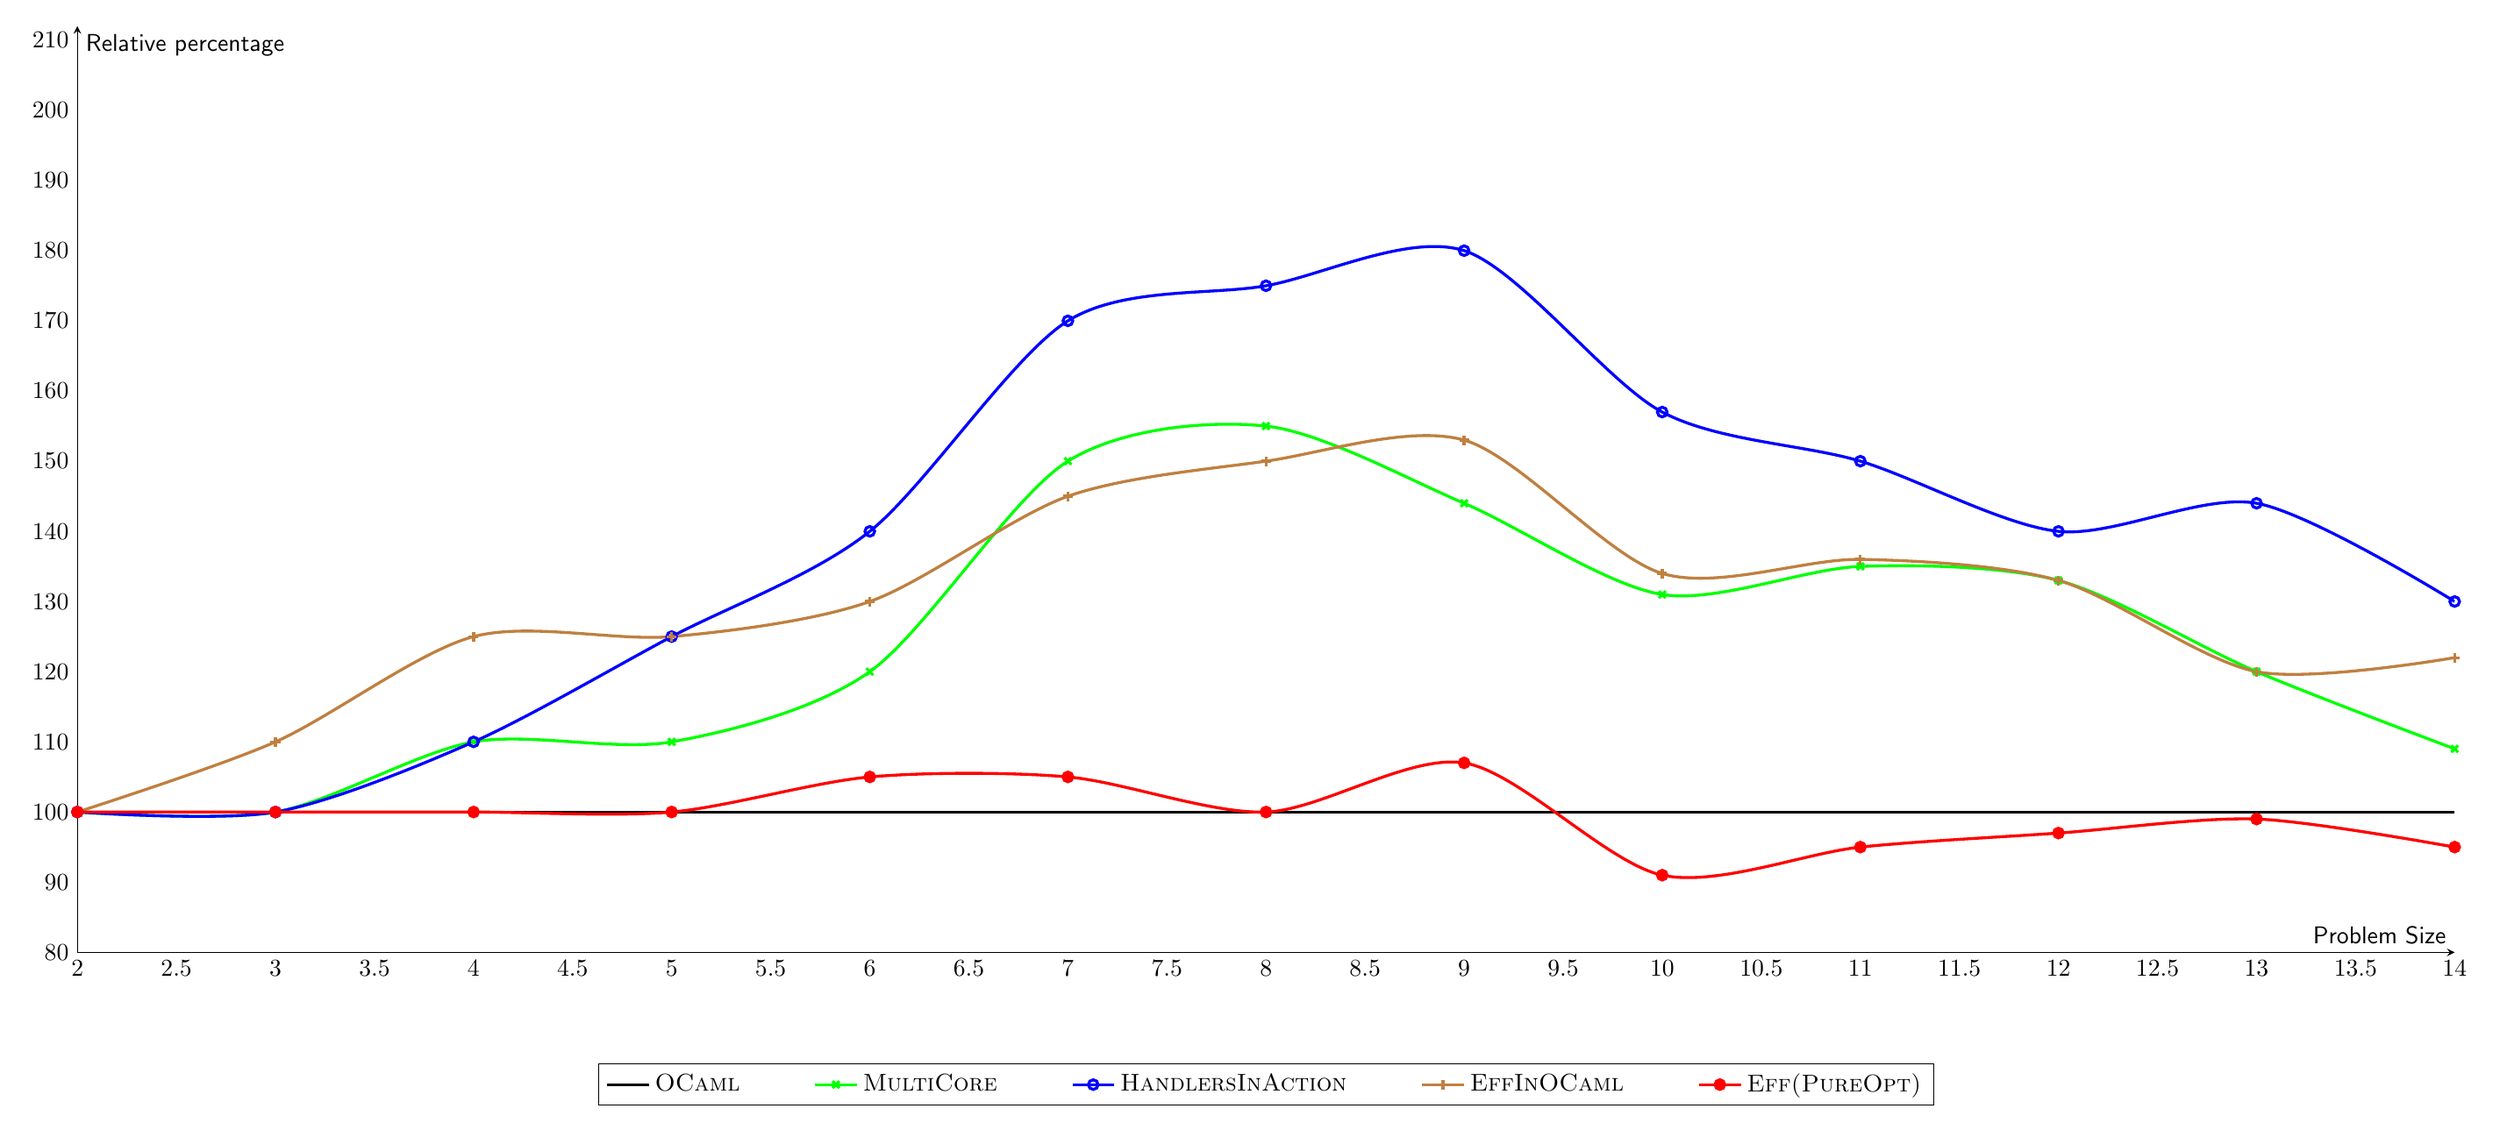
\begin{tikzpicture}
  \centering
  \begin{axis}[
        axis lines=center,
        axis on top,
        height=15cm, width=36cm,
        % bar width=0.4cm,
        % ymajorgrids, tick align=inside,
        major grid style={draw=white},
        enlarge y limits={value=.1,upper},
        ymin=80, ymax=200,
        axis x line*=bottom,
        axis y line*=left,
        % xtick = data,
        y axis line style={opacity=1},
        tickwidth=0pt,
        enlarge x limits=false,
        legend style={
            at={(0.5,-0.12)},
            anchor=north,
            legend columns=-1,
            /tikz/every even column/.append style={column sep=1cm},
            %font = \footnotesize
        },
        ylabel={Relative percentage},
        xlabel={Problem Size},
           % symbolic x coords={
           % 0,
           % 8,
           % 9,
           % 10,
           % 11,
           % 12,
           % % 13,
           % % 14
           % },
       %      nodes near coords={
       %  \pgfmathprintnumber{\pgfplotspointmeta}
       % }
    ]
    %native
    \addplot [smooth,color = black, very thick] coordinates {
      (2,100)
      (3,100)
      (4,100)
      (5,100)
      (6,100)
      (7,100)
      (8,100)
      (9,100)
      (10,100)
      (11,100)
      (12,100)
      (13,100)
      (14,100)
       };
    %multicore
    \addplot [smooth,color = green, very thick, mark = x] coordinates {
      (2,100)
      (3,100)
      (4,110)
      (5,110)
      (6,120)
      (7,150)
      (8,155)
      (9,144)
      (10,131)
      (11,135)
      (12,133)
      (13,120)
      (14,109)
       };
    %HIA
   \addplot [smooth,color = blue, very thick, mark = o] coordinates {
      (2,100)
      (3,100)
      (4,110)
      (5,125)
      (6,140)
      (7,170)
      (8,175)
      (9,180)
      (10,157)
      (11,150)
      (12,140)
      (13,144)
      (14,130)
       };
    %EffectsinOcaml
   \addplot [smooth,color = brown, very thick, mark = +] coordinates {
      (2,100)
      (3,110)
      (4,125)
      (5,125)
      (6,130)
      (7,145)
      (8,150)
      (9,153)
      (10,134)
      (11,136)
      (12,133)
      (13,120)
      (14,122)
       };
    %PureOpt
   \addplot [smooth,color = red, very thick, mark = *] coordinates {
      (2,100)
      (3,100)
      (4,100)
      (5,100)
      (6,105)
      (7,105)
      (8,100)
      (9,107)
      (10,91)
      (11,95)
      (12,97)
      (13,99)
      (14,95)
       };

    \legend{\ocaml, \textsc{MultiCore}, \textsc{HandlersInAction}, \textsc{EffInOCaml}, \textsc{\eff}\textsc{(PureOpt)}}
  \end{axis}
  \end{tikzpicture}
%  }
%\caption{Results of running N-Queens for all solutions on multiple systems}
%\label{fig:systemsall}
%\end{figure}

%----------------------------------------------------------------------------------------
%	CONCLUSIONS
%----------------------------------------------------------------------------------------

\color{SaddleBrown} % SaddleBrown color for the conclusions to make them stand out

\section*{Conclusions}

%\begin{itemize}
%\item Pellentesque eget orci eros. Fusce ultricies, tellus et pellentesque fringilla, ante massa luctus libero, quis tristique purus urna nec nibh. Phasellus fermentum rutrum elementum. Nam quis justo lectus.
%\item Vestibulum sem ante, hendrerit a gravida ac, blandit quis magna.
%\item Donec sem metus, facilisis at condimentum eget, vehicula ut massa. Morbi consequat, diam sed convallis tincidunt, arcu nunc.
%\item Nunc at convallis urna. isus ante. Pellentesque condimentum dui. Etiam sagittis purus non tellus tempor volutpat. Donec et dui non massa tristique adipiscing.
%\end{itemize}

\color{DarkSlateGray} % Set the color back to DarkSlateGray for the rest of the content

%----------------------------------------------------------------------------------------
%	FORTHCOMING RESEARCH
%----------------------------------------------------------------------------------------

\section*{Forthcoming Research}


 %----------------------------------------------------------------------------------------
%	REFERENCES
%----------------------------------------------------------------------------------------

\nocite{*} % Print all references regardless of whether they were cited in the poster or not
\bibliographystyle{plain} % Plain referencing style
\bibliography{main} % Use the example bibliography file sample.bib

%----------------------------------------------------------------------------------------
%	ACKNOWLEDGEMENTS
%----------------------------------------------------------------------------------------

\section*{Acknowledgements}

I would like to thank Amr Hany Saleh for his continuous guidance and help. I would also like to thank Matija Pretnar for his support during my research.

%----------------------------------------------------------------------------------------

\end{multicols}
\end{document}